\subsection*{Association Networks}
\addcontentsline{toc}{subsection}{Association Networks}%
{\color{red}Beyond a simple network graph representation of historical production data, the formation of association rules networks is an insightful graph-based framework combining the tools: association rules and complex networks, as Merten et al. (2020) performed in their article~\cite{MERTEN2020}. The relevant pipeline considers sequentially revealed events of a data set.} It outputs a graph demonstrating the non-random occurrence of specific events together among the complete set that took place consecutively in the production period.

Assume we have an arbitrarily created manufacturing data set with chronological order, $D$, consists of $k$ sequences and $n$ events with Feature-A values and sequence id's included as given in Table~\ref{Tab:D-dataset}.
\renewcommand{\arraystretch}{1.1}
\begin{table}[ht!]
	\centering
	\setlength{\arrayrulewidth}{0.75pt}% 
	\begin{tabular}{|c|ccc|c|}
		\hline \rowcolor[HTML]{FFFFC7}
		Event\_ID && Feature-A && Sequence\_ID   \\ \hline
		1 	      && 280  	&& 1 		   	  \\
		2 		  && 250	&& 1 		   	  \\
		3 	      && 890	&& 2 		      \\
		4 		  && 850	&& 2 		      \\
		5 	      && 650	&& 2   		      \\
		6 	      && 745	&& 2 		      \\
		7 		  && 795	&& 2 		      \\
		8 		  && 150	&& 3 		      \\
		\vdots	  && \vdots && \vdots 	      \\
		n-4 	  && 940  	&& k-1	 	      \\
		n-3 	  && 540  	&& k			  \\
		n-2 	  && 520	&& k 		      \\
		n-1       && 630	&& k 		      \\
		n 		  && 610	&& k 		      \\ \hline
	\end{tabular}
	\caption{Arbitrary Manufacturing Data Set $D$.}
	\label{Tab:D-dataset}
\end{table}

By looking at such a data set, one can say the events with Feature-A values: $890$, $850$, $650$, $745$, $795$ or $540$, $520$, $630$, $610$ are positioned in common sequences and close to each other; thus, they are produced together and likely occur in the identical sequences. As a further argument, the conclusion mentioned above is probably a deliberate planning choice based on the related constraints acting on the manufacturing process performance. However, extracting such implicit knowledge is not a simple task for large and complicated real-life manufacturing data. For example, such a data set may consist of more than $300,000$ events and is likely to have various events aggregated randomly in its large sequence groups.

We extract the association rule from the set of production sequences to distinguish statistically unexpected occurrences from the non-random ones in production sequences and assess the complexity of production patterns. The association rule measure, known as " Lift ", was picked with a similar approach as Merten et al. (2020) applied in their article~\cite{MERTEN2020}. It was calculated for every possible pairwise subset of Feature-A values belonging to the events in identical production sequences. The Lift can be computed as the ratio of pair items joint probability divided by the multiplication of each item's marginal probability as
\begin{equation} %\tag{1}
	Lift(A\leftrightarrow B)=\frac{P(A,B)}{P(A)*P(B)}.
	\label{lift}
\end{equation}
\myequations{Lift Formula}
In the case of $Lift(A\leftrightarrow B)> 1$, B occurs likely if A occurs while $Lift(A\leftrightarrow B)< 1$, B unlikely occurs if A occurs. Indication of random and non-random co-occurrences as $0$ and $1$ in an adjacency matrix will provide the data structure to form an association network, as shown in Fig.~\ref{figure-adjacency_graph}.

 \begin{figure}[!ht]
	\begin{center}
		\makebox[\textwidth]{
			\centering
			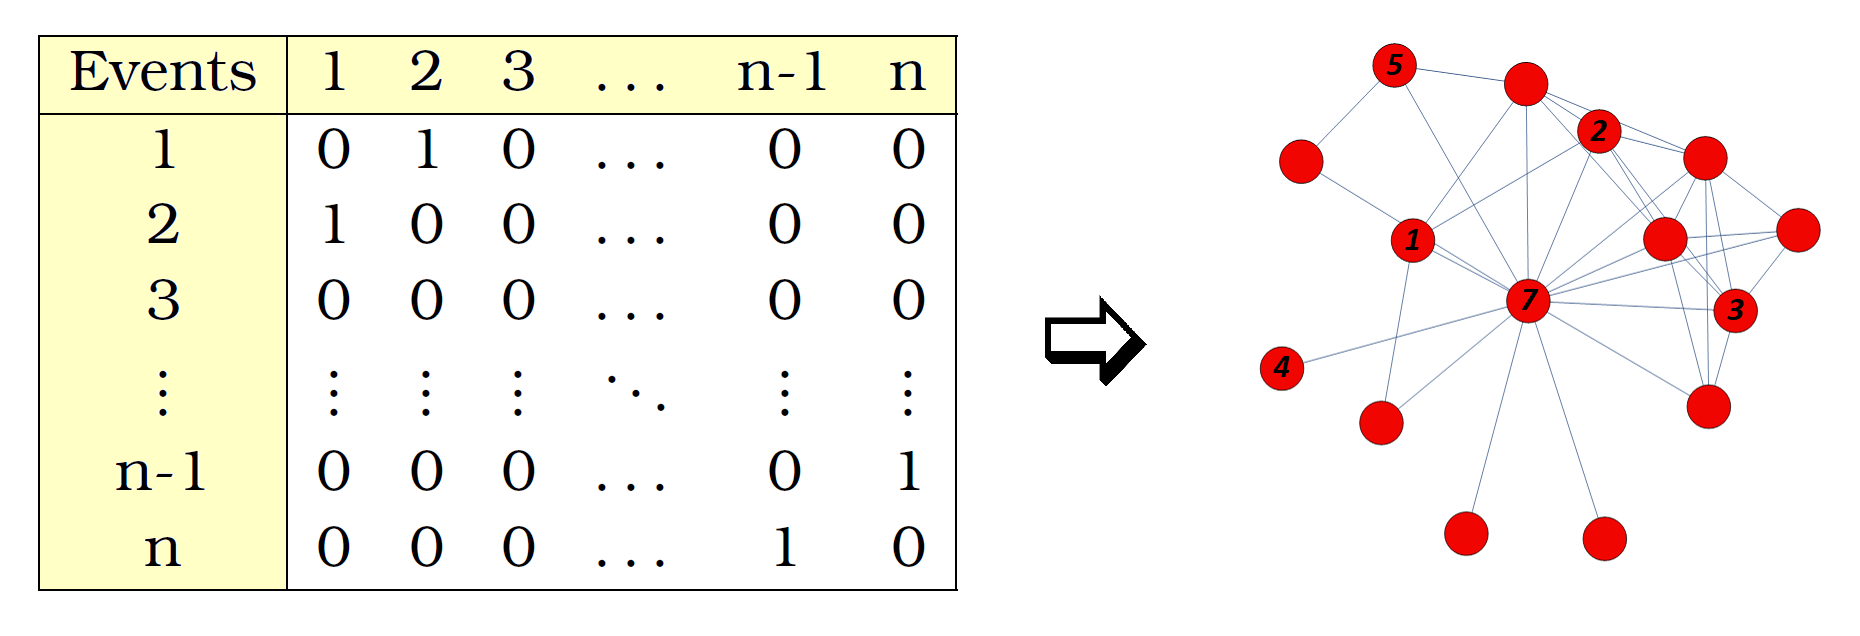
\includegraphics[width=0.7\linewidth]{../images/methodology-association-networks-adjacency_graph.png}}
		\caption{An Arbitrary Representation for Adjacency Matrix and Its Graph.}
		\label{figure-adjacency_graph}
	\end{center}
\end{figure}

%\begin{table}[]
%	\begin{tabular}{|c|cccccc|}
%		\hline
%		Events & 1   & 2   & 3   & \dots & n-1 & n   \\ \hline
%		1      & 0   & 1   & 0   & \dots & 0   & 0   \\
%		2      & 1   & 0   & 0   & \dots & 0   & 0   \\
%		3      & 0   & 0   & 0   & \dots & 0   & 0   \\
%		\vdots & \vdots & \vdots & \vdots & \ddots & \vdots & \vdots \\
%		n-1    & 0   & 0   & 0   & \dots & 0   & 1   \\
%		n      & 0   & 0   & 0   & \dots & 1   & 0   \\ \hline
%	\end{tabular}
%\end{table}